
\section{InfoRM: Ослабление взлома вознаграждения в обучение с подкреплением на основе человеческой обратной связи через информационно-теоретическое моделирование вознаграждения}

\subsection{Ключевые идеи}

В статье~\cite{miao2024inform} предлагается метод \textbf{InfoRM}~-- информационно-теоретическая модель вознаграждения,
предназначенная для снижения эффекта переоптимизации вознаграждения
в рамках обучения с подкреплением на основе человеческой обратной связи.

Основная идея заключается в том, что переоптимизация возникает из-за неверного обобщения вознаграждения~-- прокси-модель вознаграждения начинает использовать признаки, не отражающие человеческие предпочтения.
Чтобы этого избежать, InfoRM вводит информационное бутылочное горлышко (см. Рис~\ref{fig:architecture6}),
позволяющее сохранять в латентном представлении только ту информацию,
которая связана с реальными человеческими оценками.

\begin{figure}[h!]
\centering
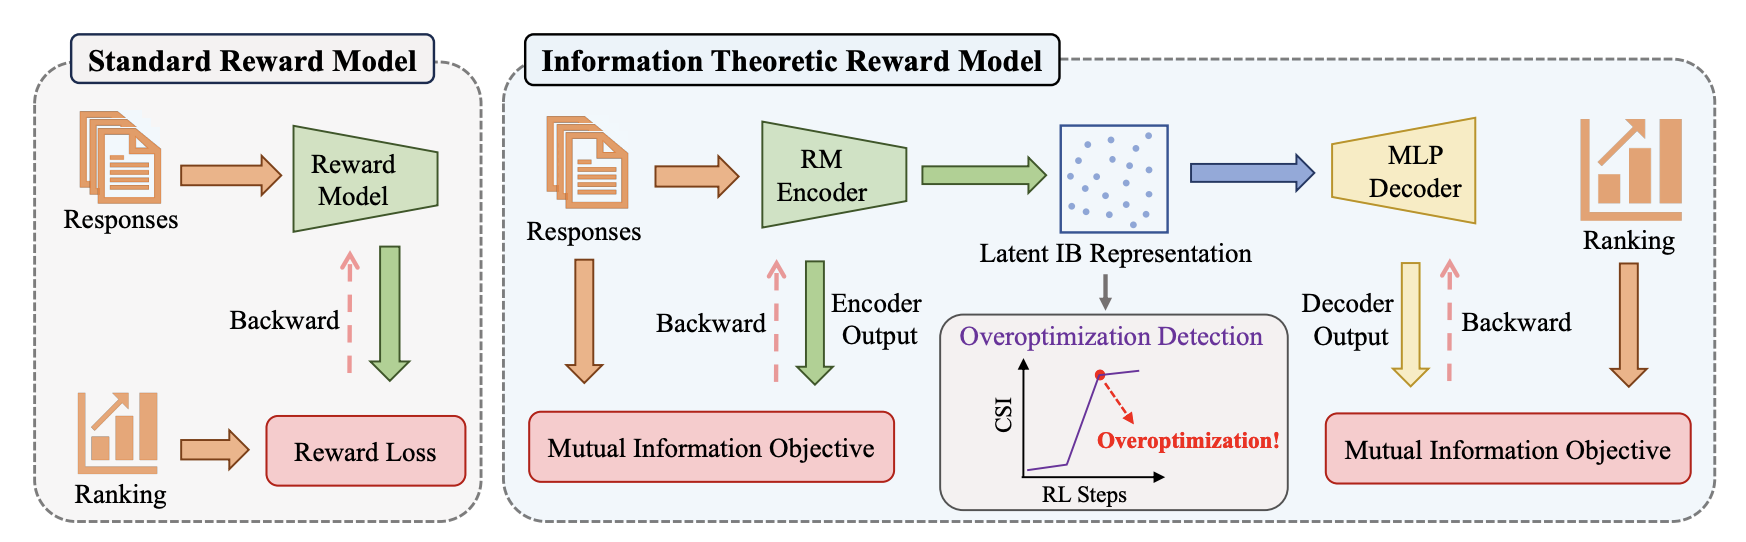
\includegraphics[width=0.95\textwidth]{images/Comparison_standard_RM_and_model_InfoRM.png}
\caption{Сравнение стандартной модели вознаграждения и информационно-теоретической модели (InfoRM)}
\label{fig:architecture6}
\end{figure}

\subsection{Математическое описание метода}

Основная идея InfoRM~-- представить процесс моделирования вознаграждения в терминах взаимной информации между входом $X$, латентным представлением $S$ и человеческими предпочтениями $Y$.

Оптимизационная цель формулируется как:

\begin{equation}
\max_{\theta} J(\theta) = \max_{\theta} \Big( I(S; Y) - \beta I(X; S | Y) \Big),
\end{equation}

где $I(S; Y)$ отражает информативность латентного представления относительно человеческих предпочтений,
$I(X; S | Y)$ штрафует нерелевантную информацию,
а $\beta$ регулирует компромисс между этими двумя компонентами.

Так как взаимную информацию напрямую вычислить сложно, используется вариационная нижняя граница:

\begin{equation}
J(\phi, \psi) \ge J_{\mathrm{VLB}}(\phi, \psi) = \mathbb{E}{(x, y) \sim \mathcal{D}}
\Big[ J{\mathrm{pref}} - \beta J_{\mathrm{bott}} \Big],
\end{equation}

где

\begin{equation}
\begin{aligned}
J_{\mathrm{pref}} &= \int p_{\phi}(s|x) \log q_{\psi}(y|s) ds, \\
J_{\mathrm{bott}} &= \mathrm{KL}\big[p_{\phi}(S|x), r(S)\big].
\end{aligned}
\end{equation}

Таким образом, InfoRM обучается не просто предсказывать ранжирование ответов, а строить устойчивое латентное представление, минимизирующее влияние шумовых факторов.

\subsection{Алгоритм}

На Рис.~\ref{fig:architecture6} видно, что архитектура InfoRM включает два ключевых компонента~-- кодировщик (RM Encoder) и декодер (MLP Decoder).

\paragraph{Генерация данных.}
SFT-модель создаёт пары ответов $(x^w, x^l)$, которые оцениваются эталонной моделью. Эта модель полностью соответствует человеческим оценкам модели вознагражения.

\paragraph{Энкодер InfoRM}
Кодировщик преобразует входные ответы в латентное представление $S$,
обучаясь по принципу информационного бутылочного горлышка.

\paragraph{Оптимизация.}
Используется следующая аппроксимация целевой функции:
\begin{equation}
\begin{aligned}
L_{\mathrm{pref}} &= \log \sigma\Big(g_{\psi}(h_{\phi}(x^w, \epsilon^w)) - g_{\psi}(h_{\phi}(x^l, \epsilon^l))\Big), \\
L_{\mathrm{bott}} &= \mathrm{KL}\big[p_{\phi}(S|x^w), r(S)\big] + \mathrm{KL}\big[p_{\phi}(S|x^l), r(S)\big], \\ \\
& \text{где } h_{\phi}(x, \epsilon) = f_{\phi}^{\mu}(x) + f_{\phi}^{\sigma}(x)\epsilon, \epsilon \sim \mathcal{N}(0, I).
\end{aligned}
\end{equation}

\paragraph{Модуль обнаружения переоптимизации.}
Анализируется распределение латентных векторов $S$.
Появление выбросов фиксируется через индекс разделения кластеров CSI:
\begin{equation}
\begin{aligned}
c_i &= \frac{1}{|C_i|} \sum_{x \in C_i} x, \\
d_i &= \min_{s \in S} | c_i - s |, \\
CSI &= \sum_{i=1}^{n} |C_i| \cdot d_i.
\end{aligned}
\end{equation}
Резкий рост индекса разделения кластеров сигнализирует о начале переоптимизации и может служить критерием для ранней остановки обучения с подкреплением на основе человеческой обратной связи.

\subsection{Наборы данных}

\paragraph{Симуляционные эксперименты.} Для оценки эффективности InfoRM в контролируемых условиях использовались данные из \emph{AlpacaFarm}~\cite{dubois2023alpacafarm}, где формируются пары инструкций и ответов с предпочтениями, сгенерированными эталонной моделью.  

Для обучения политики и прокси-модели вознаграждения применялись модели семейства \emph{Pythia} различного масштаба~-- 70M, 410M и 1.4B параметров. 


Такой выбор обеспечивает единообразие архитектуры и позволяет исследовать влияние размера модели на устойчивость к переоптимизации.

\paragraph{Реальные эксперименты.} В экспериментах на реальных данных InfoRM оценивался на нескольких задачах:

\begin{itemize}
    \item Anthropic-RLHF-HH~\cite{anthropic_hh_rlhf}~-- крупномасштабный корпус диалогов, включающий полезные и безопасные  ответы, используемый для обучения и тестирования моделей вознаграждения в задачах общения.  
    \item Reddit TL;DR~\cite{trl_tldr}~-- датасет для задачи суммаризации текстов, применяемый на всех этапах обучения с подкреплением на основе человеческой обратной связи: предварительное обучение (SFT), моделирование вознаграждения и оптимизация политики.  
    \item Flan~\cite{openorca_flan}, Vicuna~\cite{vicuna2023}, Koala~\cite{koala2023}~-- дополнительные наборы данных для оценки обобщающей способности InfoRM, включающие инструкции и ответы из различных источников (out-of-distribution).  
\end{itemize}



\subsection{Метрики}

Для количественной оценки эффективности InfoRM и степени переоптимизации вознаграждения использовались следующие метрики:

\begin{itemize}
    \item Gold Score~-- оценка качества ответов по «золотой» модели вознаграждения (gold RM), отражающая истинные человеческие предпочтения.
    
    \item Proxy Score~-- оценка по прокси-модели вознаграждения (proxy RM), служащая оптимизационной целью в процессе RLHF.
    
    \item KL-дивергенция — мера отклонения распределения политики от исходной SFT-модели, контролирующая степень сдвига поведения при обучении с подкреплением.
    
    \item Индекс CSI (Cluster Separation Index)~-- разработанный в данной работе количественный индикатор переоптимизации, вычисляемый на основе распределения латентных представлений в пространстве информационного бутылочного горлышка (IB).
    
    \item Win / Tie / Lose Ratio~-- относительные доли побед, ничьих и поражений в парных сравнениях ответов моделей, оцениваемых GPT-4; используется для итоговой оценки качества с точки зрения человеческих предпочтений.
\end{itemize}

\subsection{Модели}

В экспериментальной части использовались следующие модели и конфигурации:

\begin{itemize}
    \item Модель предварительного обучения (SFT)~-- \emph{Vicuna-7B-v1.5}~\cite{vicuna2023}, основанная на архитектуре \emph{LLaMA2-7B}~\cite{llama2_2023}; применяется в качестве базовой модели, обученной по инструкциям с использованием человеческой обратной связи.
    
    \item Модель политики~-- \emph{Pythia-1.4B}~\cite{bai2022helpfulharmless}; используется в симуляционных экспериментах на этапе обучения с подкреплением по человеческой обратной связи для оптимизации поведения на основе модели вознаграждения.
    
    \item Прокси-модель вознаграждения~-- семейство моделей \emph{Pythia}~\cite{bai2022helpfulharmless} различного масштаба (70M, 410M, 1.4B параметров), дополненных выходным MLP-слоем, который формирует скалярную оценку вознаграждения.
    
    \item Эталонная модель вознаграждения~-- \emph{Vicuna-7B-v1.5}, обученная по протоколу \emph{AlpacaFarm}~\cite{dubois2023alpacafarm} и используемая в качестве эталонной модели человеческих предпочтений в симуляционных экспериментах
    
    \item Базовые методы для сравнения:
    \begin{itemize}
        \item Стандартная модель вознаграждения~-- классическая прокси-модель, обучаемая по парным человеческим предпочтениям.  
        \item Стандартная модель вознаграждения с KL-регуляризацией~-- модификация, где к функции потерь добавлен штраф Кульбака–Лейблера для ограничения отклонения политики от SFT-модели.  
        \item Ансамблевая модель вознаграждения (Ensemble RM)~-- комбинация нескольких прокси-моделей для повышения устойчивости оценки.  
        \item Средневзвешенная модель вознаграждения (WARM)~-- агрегирование весов нескольких моделей вознаграждения для сглаживания переобучения и уменьшения переоптимизации.  
    \end{itemize}
\end{itemize}

\subsection{Результаты}

Результаты экспериментов показывают, что предложенная информационно-теоретическая модель вознаграждения \emph{InfoRM} эффективно предотвращает явление переоптимизации вознаграждения даже при наличии значительного уровня шума в данных обучения (до 25\% ошибочных меток предпочтений). 


В сравнении со стандартной моделью вознаграждения и её вариантом с KL-регуляризацией, \emph{InfoRM} демонстрирует существенно более высокие значения оценки эталонной модели человеческих предпочтений и обеспечивает стабильную динамику обучения в процессе обучения с подкреплением на основе человеческой обратной связи, что повышает общую эффективность обучения с подкреплением.  

Дополнительно показано, что \emph{InfoRM} обладает лучшей способностью к обобщению на данных, находящихся вне исходного распределения. В частности, при тестировании на корпусе \emph{Flan} (out-of-distribution) модель сохраняет стабильное качество, в то время как стандартная модель вознаграждения демонстрирует заметное ухудшение результатов.  

Наконец, предложенный авторами индекс разделения кластеров показал себя как надёжный индикатор возникновения переоптимизации. Его использование позволяет реализовать механизм автоматической ранней остановки обучения, предотвращая переобучение и деградацию качества модели на поздних этапах обучения с подкрепления на основе человеческой обратной связи.
